% -*- coding: utf-8 -*-
%%
%%  本模板可以使用以下两种方式编译:
%%     1. PDFLaTeX
%%     2. XeLaTeX [推荐]
%%  注意:
%%    1. 在改变编译方式前应先删除 *.toc 和 *.aux 文件,
%%       因为不同编译方式产生的辅助文件格式可能并不相同。

% \documentclass{cumcmart}
\documentclass[nocover]{cumcmart}%%%切换到无封面的版本,有些区域不允许前面的承诺页用pdf格式,可以用此去掉。



\begin{document}

\xuanti{A}
%\school命令用于在承诺书上显示学校名称。按要求,此处应填写全称
\school{长江大学}
%以下命令分别显示队员及指导教师姓名
\numbers{2017000}%参赛报名号
\authorone{孔庆亮}
\authortwo{朱艳玲}
\authorthree{刘艳}
\advisor{数模指导组}

%\theyear{2017}
\theday{07}%填写当月的具体日期

\title{Title}

\maketitle

\begin{cnabstract}%此处没有采用sbstract命名,是为了将来如果要加入英文摘要时扩展的方便


\cnkeywords{符号秩检验,方差检验,因子分析,聚类分析,}
\end{cnabstract}

\newpage
%\tableofcontents\newpage%增加目录,要不要都可以。不想要的话,就在本行前加“%”(英文的百分号)


\section{问题重述}
确定葡萄酒质量时一般是通过聘请一批有资质的评酒员进行品评。每个评酒员在对葡萄酒进行品尝后对其分类指标打分,然后求和得到其总分,从而确定葡萄酒的质量。酿酒葡萄的好坏与所酿葡萄酒的质量有直接的关系,葡萄酒和酿酒葡萄检测的理化指标会在一定程度上反映葡萄酒和葡萄的质量。

利用附件一、附件二和附件三所给的数据,解决以下问题:
    \begin{enumerate}
        \item 分析两组评酒员的评价结果有无显著性差异,如果有则需要确定哪一组评酒员的结果更可信;
        \item 根据酿酒葡萄的理化指标和葡萄酒的质量,对这些酿酒葡萄进行分级;
        \item 酿酒葡萄与葡萄酒的理化指标,寻找其中的联系;
        \item 分析酿酒葡萄和葡萄酒的理化指标对葡萄酒质量的影响,并论证能否用葡萄和葡萄酒的理化指标来评价葡萄酒的质量。
    \end{enumerate}

\section{建模分析}

    \subsection{模型假设}

    对于葡萄和葡萄酒的理化指标与葡萄和葡萄酒的质量所建立的模型模型,我们提出了如下的合理假设:
    \begin{enumerate}
        \item 未考虑到的酿酒葡萄理化指标不会影响葡萄酒的质量;
        \item 各位评酒员打分彼此之间没有影响;
        \item 抽出葡萄样品能代替一种葡萄;
        \item 评酒结果采取加分制;
        \item 附件2中给出的葡萄和葡萄酒理化指标都准确可靠;
        \item 
        \item 
    \end{enumerate}

    \subsection{记号说明}

    \begin{table}[!htbp]
        \centering
        \begin{tabular}{cl}
        \toprule
        \multicolumn{2}{c}{\large 模型记号说明}\\
        \midrule
            ${P_i}$         &   第i组评酒员整体,${i = 1,2}$    \\
            ${J_{i}^{k}}$ &   $k$ 葡萄酒的第 $i$ 样品($k=1,\text{红葡萄酒;} k=2,\text{白葡萄酒}$)  \\ 
             &  \\
             &  \\
            

        \bottomrule
        \end{tabular}
        \caption{模型记号说明}
    \end{table}

    \subsection{问题分析}

        \subsubsection{缺省值和异常值处理}
        通过MATLAB数据预处理,发现“第一组红葡萄酒品尝评分表中(76, F)数据缺失,而第一组白葡萄酒品尝评分表中(233, J)及(298, L)数据异常,为此我们对数据进行预处理。使用异常值所在的项目的其他数据的均值去替代,即消除异常数据对其他数据的影响
。
        \subsubsection{可靠性分析}
        因为两组品酒员对酒样的评分是成对比较,且对评分并不要求成对数据之差服从正态分布,只要求对称分布,再有葡萄酒质量评判的分布的不确定性,故我们采用统计学中 Wilcoxon 符号秩检验来解释两组评酒员对葡萄酒的评价有无显著性差异。

        如果两组评酒员对葡萄酒的评价有显著性差异,就需要确定哪一组的评价更可信,因此我们两组的方差,对两组评酒员的评价数据进行置信度分析。利用MATLAB的信度分析功能,分别对第一组和第二组评分进行可信度分析,最后通过图形直观的反映结果。

        \subsubsection{因子分析、聚类分析}
        由于酿酒葡萄的理化指标繁杂,彼此之间相互联系,


        \subsubsection{多元逐步回归分析}

    \subsection{建立模型}

        \subsubsection{符号秩检验模型的建立}
    将两组评酒员分别看作两个整体 ${P_1}$、${P_2}$ ,对每个红葡萄酒样品 ${J_{i}^{1}}$ 每个白葡萄酒样品 ${J_{i}^{2}}$进行评价,${P_1}$ 对每个红葡萄酒的样品 ${J_{i}^{1}}$ 的评价结果通过组内每一位品酒员的评分 ${x_{ij}^{1}}$ 的均值 $\bar{x}_{i}^1 = \frac{1}{10}\sum\limits_{j=1}^{10}x_{ij}^{1}$来刻画,对每个白葡萄酒的样品 ${J_{i}^{2}}$ 的评价结果通过组内每一位品酒员的评分 ${x_{ij}^{2}}$ 的均值 ${\bar{x}_{i}^{2}} = \frac{1}{10}\sum\limits_{j=1}^{10}x_{ij}^{1}$来刻画,同样 ${P_2}$ 对每个红葡萄酒的样品 ${J_{i}^{1}}$ 的评价结果用均值 ${\bar{y}_{i}^{1}} = \frac{1}{10}\sum\limits_{j=1}^{10}y_{ij}^{1}$,对每个白葡萄酒的样品 ${J_{i}^{2}}$ 的评价结果用均值 ${\bar{y}_{i}^{2}} = \frac{1}{10}\sum\limits_{j=1}^{10}y_{ij}^{2}$来刻画,从而得到两组评酒员对每种样品酒的评价结果,建立两组评酒员对红葡萄酒和白葡萄酒的评价。

    对酒样品 ${J_i}$,${J_2}$ 分别得到一对数据。葡萄酒质量是其外观、香气、口味、典型性的综合表现\cite{1},可知两对数据之间的差异由多种因素引起,由于不仅酒样品 ${J_{i}^{1}}$、${J_{i}^{2}}$ 的特性有广泛的差异,而且评酒员存在感官评价的异质性\cite{2},就不能将一组评酒员对27种红葡萄酒或者28种白葡萄酒的评价结果看成是同分布随机变量。为鉴定他们的评价结果有无显著性差异,可使用基于成对数据的逐对比较法,以红葡萄酒样品为例,有27对相互独立的评价结果:${(X_1,Y_1),(X_2,Y_2),\ldots,(X_{27},Y_{27})}$,令${D_1 = X_1 - Y_1,D_2 = X_2 - Y_2,\ldots,D_{27} = X_{27} - Y_{27}}$,则${D_1,D_2,\ldots,D_{27}}$相互独立,我们对 ${D_1,D_2,\ldots,D_{27}}$ 进行符号秩和检验。


        \subsubsection{暂定}


        \subsubsection{多元逐步回归分析模型}




    \subsection{模型求解和分析}

        \subsubsection{符号秩检验模型的求解}
        将附件一中的数据使用MATLAB整合、分析、处理,可得两组的葡萄酒品尝评分的均值和方差的总表。

        利用MATLAB的 \verb| signrank | 符号秩检验函数,就可以得到
        \begin{verbatim}
            >>  [p,h] = signrank(red1aver,red2aver)

            >>  p =  0.0105
            >>  h =  1

            >>  [p,h] = signrank(write1aver,write2aver)

            >>  p = 0.0372
            >>  h = 1

        \end{verbatim}

        两个 $h$ 都为 $1$ ,即两组评酒员的评价结果均有显著性差异,再由两组方差总值与方差分析图,可以得到第二组的评分结果更可信。

    \begin{table}[!htbp]
    \centering
        \begin{tabular}{ccccccccccccccc}
        \toprule
        \multicolumn{3}{c}{第一组评酒员} &  & \multicolumn{3}{c}{第二组评酒员} & 酒 & \multicolumn{3}{c}{第一组评酒员} &  & \multicolumn{3}{c}{第二组评酒员} \\
        \cmidrule{1-3}  \cmidrule{5-7}   \cmidrule{9-11}  \cmidrule{13-15}
            总分    &    均值   &   方差   &  &  方差     &    均值   &  总分   & 号  & 总分    &    均值   &   方差   &  &  方差     &    均值   &  总分\\
        \midrule

            627  &  62.70  &  92.90   &  &  81.87  &  68.10  &  681  &  1   &  820  &   82.00  &  92.222   &   &  25.88   &   77.90   &   779   \\
            803  &  80.30  &  39.78   &  &  16.22  &  74.00  &  740  &  2   &  742  &   74.20  &  201.06   &   &  49.07   &   75.80   &   758   \\
            804  &  80.40  &  45.82   &  &  30.71  &  74.60  &  746  &  3   &  853  &   85.30  &  365.12   &   &  142.48  &   75.60   &   756   \\
            686  &  68.60  &  108.04  &  &  41.28  &  71.20  &  712  &  4   &  794  &   79.40  &  44.711   &   &  42.10   &   76.90   &   769   \\
            733  &  73.30  &  62.01   &  &  13.65  &  72.10  &  721  &  5   &  710  &   71.00  &  126.44   &   &  26.28   &   81.50   &   815   \\
            722  &  72.20  &  59.73   &  &  21.12  &  66.30  &  663  &  6   &  684  &   68.40  &  162.71   &   &  22.72   &   75.50   &   755   \\
            715  &  71.50  &  103.61  &  &  62.67  &  65.30  &  653  &  7   &  775  &   77.50  &  39.166   &   &  42.18   &   74.20   &   742   \\
            723  &  72.30  &  44.01   &  &  65.11  &  66.00  &  660  &  8   &  714  &   71.40  &  183.60   &   &  31.12   &   72.30   &   723   \\
            815  &  81.50  &  32.94   &  &  25.73  &  78.20  &  782  &  9   &  729  &   72.90  &  92.766   &   &  106.26  &   80.40   &   804   \\
            742  &  74.20  &  30.40   &  &  36.17  &  68.80  &  688  &  10  &  743  &   74.30  &  212.67   &   &  70.40   &   79.80   &   798   \\
            701  &  70.10  &  70.76   &  &  38.04  &  61.60  &  616  &  11  &  723  &   72.30  &  177.12   &   &  87.82   &   71.40   &   714   \\
            539  &  53.90  &  79.65   &  &  25.12  &  68.30  &  683  &  12  &  633  &   63.30  &  115.78   &   &  140.04  &   72.40   &   724   \\
            746  &  74.60  &  44.93   &  &  15.28  &  68.80  &  688  &  13  &  659  &   65.90  &  170.76   &   &  46.77   &   73.90   &   739   \\
            730  &  73.00  &  36.00   &  &  23.15  &  72.60  &  726  &  14  &  720  &   72.00  &  114.22   &   &  15.88   &   77.10   &   771   \\
            587  &  58.70  &  85.56   &  &  41.34  &  65.70  &  657  &  15  &  724  &   72.40  &  131.60   &   &  54.04   &   78.40   &   784   \\
            749  &  74.90  &  18.10   &  &  20.10  &  69.90  &  699  &  16  &  740  &   74.00  &  178.00   &   &  82.23   &   67.30   &   673   \\
            793  &  79.30  &  88.01   &  &  9.16   &  74.50  &  745  &  17  &  788  &   78.80  &  144.17   &   &  38.46   &   80.30   &   803   \\
            601  &  60.10  &  42.76   &  &  50.26  &  65.40  &  654  &  18  &  731  &   73.10  &  156.54   &   &  30.23   &   76.70   &   767   \\
            786  &  78.60  &  47.37   &  &  55.15  &  72.60  &  726  &  19  &  722  &   72.20  &  46.40    &   &  26.04   &   76.40   &   764   \\
            792  &  79.22  &  15.25   &  &  39.06  &  75.80  &  758  &  20  &  778  &   77.80  &  64.40    &   &  50.04   &   76.60   &   766   \\
            771  &  77.10  &  116.10  &  &  35.51  &  72.20  &  722  &  21  &  764  &   76.40  &  172.71   &   &  64.40   &   79.20   &   792   \\
            772  &  77.20  &  50.62   &  &  24.26  &  71.60  &  716  &  22  &  710  &   71.00  &  138.66   &   &  53.60   &   79.40   &   794   \\
            856  &  85.60  &  32.48   &  &  24.76  &  77.10  &  771  &  23  &  759  &   75.90  &  43.65    &   &  11.60   &   77.40   &   774   \\
            780  &  78.00  &  74.88   &  &  10.72  &  71.50  &  715  &  24  &  733  &   73.30  &  111.12   &   &  38.54   &   76.10   &   761   \\
            692  &  69.20  &  64.62   &  &  43.73  &  68.20  &  682  &  25  &  771  &   77.10  &  33.87    &   &  106.50  &   79.50   &   795   \\
            738  &  73.80  &  31.28   &  &  41.55  &  72.00  &  720  &  26  &  813  &   81.30  &  72.90    &   &  102.90  &   74.30   &   743   \\
            730  &  73.00  &  49.77   &  &  20.50  &  71.50  &  715  &  27  &  648  &   64.80  &  144.40   &   &  35.56   &   77.00   &   770   \\
                 &         &          &  &         &         &       &  28  &  813  &   81.30  &  80.46    &   &  25.38   &   79.60   &   796   \\

        \midrule
                &          & 1567.49  &  & 912.34  &         &       &        &     &          &   3617.30 &   & 1568.54  &           &         \\
        \bottomrule
        \end{tabular}
        \caption{两组葡萄酒品尝评分的均值和方差}
    \end{table}
 

    \subsection{模型评价}

        \subsubsection{模型优点}
1)	

2)	

3)	

        \subsubsection{模型缺点}
1)	

2)	


%   \begin{figure}
%   \centering
%   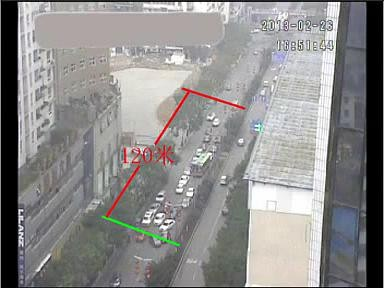
\includegraphics[width=.6\textwidth]{fig1}
%   \caption{发生事故时车流饱和状态图示}
%   \end{figure}

\begin{thebibliography}{10}

\bibitem{1} 李云. 统计分析在葡萄酒质量评价中的应用. 酿酒科技,2009.
\bibitem{2} 李华. 葡萄酒感官评价结果的统计分析方法研究. 中国食品学报,2006.

% \bibitem{1} \url{http://bbs.chinatex.org}
% \bibitem{2} \url{http://www.chinatex.org}
% \bibitem{3} Alpha Huang, \textbf{latex-notes-zh-cn}, 2014.
% \bibitem{lf}M.R.C. van Dongen,\textbf{\LaTeX-and-Friends}, 2013.
% \bibitem{figure}Keith Reckdahl,\textbf{Using Import graphics in \LaTeXe}, 1997.
% \bibitem{HM}Addison Wesley,\textbf{Higher Mathematics}, 下载地址如下\\ \url{http://media.cism.it/attachments/ch8.pdf}
\end{thebibliography}


\newpage
\appendix
\section*{附 \quad 录}


\end{document}
